\documentclass[a4paper,10pt,twocolumn]{myjarticle2}

\usepackage[dvipdfmx]{graphicx}
\usepackage{multirow}

%ルビ
\def\ruby#1#2{%
  \leavevmode \setbox0=\hbox{\mathstrut#1}\setbox1=\hbox{\tiny#2}%
  \ifdim\wd0>\wd1 \dimen0=\wd0 \else \dimen0=\wd1 \fi
  \hbox{\kanjiskip=\fill
    \vbox{\hbox to \dimen0{\tiny \hfil#2\hfil}%
       \nointerlineskip
       \hbox to \dimen0{\hfil\mathstrut#1\hfil}}}}
% <<DISPLAYSTYLE mathematical characters>>
%\newcommand{\Frac}[2]{\displaystyle\frac{\raisebox{-1.8pt}{$#1$}}{\raisebox{0.8pt}{$\:#2\:$}}}
\newcommand{\Frac}{\displaystyle\frac}
\newcommand{\Prod}{\displaystyle\prod}
\newcommand{\Sum}{\displaystyle\sum}
\newcommand{\Int}{\displaystyle\int}
\newcommand{\Sqrt}[1]{\sqrt{#1\,}}
\newcommand{\Lim}{\displaystyle\lim}
\newcommand{\Cup}{\displaystyle\bigcup}
\newcommand{\Cap}{\displaystyle\bigcap}
\newcommand{\Min}{\displaystyle\min}
\newcommand{\Max}{\displaystyle\max}
\newcommand{\Vec}[1]{\overrightarrow{#1}}
\newcommand{\Vecb}[1]{\mbox{\boldmath $#1$}}
\newcommand{\NumB}[1]{\noindent\fbox{{\large\bf#1}}\hspace{3pt}}
% <<日本式不等号>>
\makeatletter\def\le{\mathrel{\mathpalette\gl@align<}}
\def\ge{\mathrel{\mathpalette\gl@align>}}
\def\gl@align#1#2{\lower.6ex\vbox{\baselineskip\z@skip\lineskip\z@%
\ialign{$\m@th#1\hfil##\hfil$\crcr#2\crcr=\crcr}}}
\makeatother

\def\labelenumi{(\theenumi)}
\def\theenumi{\roman{enumi}}


\pagestyle{empty}

\setlength{\topmargin}{6mm}
\setlength{\oddsidemargin}{-4mm}
\setlength{\evensidemargin}{-4mm}
\setlength{\textwidth}{170mm}
\setlength{\headsep}{0pt}
\setlength{\headheight}{0pt}
\setlength{\textheight}{235mm}
\setlength{\columnsep}{5mm}

\begin{document}
\twocolumn[%
\vspace{-20mm}
\begin{center}
{\LARGE\bf ファジィシステムシンポジウム講演論文集原稿作成要領\textcircled{1}}
\vspace{2mm}\par\noindent
{\large
Instruction for Preparing Fuzzy System Symposium Manuscript\textcircled{2}}
\vspace{2mm}\par\noindent
{\large
\begin{tabular}{cc}
$\bigcirc$ あいまい　太郎$^{1}$， & あいまい　花子$^{2}$\textcircled{3}\\
$\bigcirc$ Taro Aimai$^{1}$, & Hanako Aimai$^{2}$\textcircled{4}\\
\multicolumn{2}{c}{$^{1}$ファジィ大学 \textcircled{5}}{$^{2}$SOFT 株式会社\textcircled{5}}\\
\multicolumn{2}{c}{$^{1}$Fuzzy University\textcircled{6}}{$^{2}$SOFT Corporation\textcircled{6}}\\
\end{tabular}
}\vspace{2mm}\par\noindent
\begin{minipage}{150mm}
{\small
{\bf Abstract:\textcircled{7}}
%%%%% 英文アブストラクト %%%%%
This article presents the guidelines for preparing camera-ready papers for FSS2026.
%%%%%%%%%%%%%%%%%%%%%%%%%%%%%%
\par\noindent
}
\end{minipage} \par\noindent
\end{center}
]
\section{はじめに\textcircled{8}}
以下の要領を参考に，原稿を執筆してください\cite{文献1}．
\section{用紙}
A4用紙サイズ（縦置き），上下左右のマージン（余白）をそれぞれ20mm以上に設定してください．\underline{レターサイズの原稿は受け付けません}．
\section{ページ数}
2～6ページで作成してください(奇数ページでも可)．図表の書き方は，本執筆要領を参考にしてください．本文の文字の大きさは10ポイント程度とします．
\begin{figure}[!h]
\centering
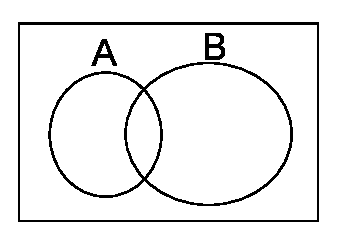
\includegraphics[scale=0.6]{sample.eps}
\caption{サンプル図} \label{figData}
\end{figure}
\begin{table}[!h]
\centering
\caption{サンプル表}
\begin{tabular}{|c|c|c|c|c|}
\hline
\multicolumn{2}{|c|}{\multirow{2}{*}{$u_k$}} & \multicolumn{3}{|c|}{$y_k$} \\ \cline{3-5}
\multicolumn{2}{|c|}{} & N & Z & P \\ \hline
\multirow{3}{*}{$r_k$} & N & N & N & Z \\ \cline{2-5}
 & Z & P & Z & N \\ \cline{2-5}
 & P & P & P & P \\ \hline
\end{tabular}
\end{table}
\section{注意事項}
原稿執筆に当たっては特に以下の点に留意してください．
\begin{enumerate}
\item 用紙サイズ（A4），マージンサイズ（20mm以上）を\underline{必ず確認}してください．
\item ヘッダやフッタには\underline{何も書かない}でください（ページ番号は書かない）．
\item 著者欄では，和文著者名，英文著者名，著者の所属名（和文名と英文名を並べて書く）の順に記載してください．
\item 当日発表を行う著者名に丸印（$\bigcirc$）をつけてください．
\item 図表などがマージン部分に\underline{はみ出さない}よう注意してください．
\item CD-ROMには著者がPDF化した原稿を掲載します．PDFファイルは\underline{書き込み可}の設定にしてください（ページ番号等を付加するため）．
\item PDF化の際には，\underline{フォントを埋め込んで}ください．
\item 原稿は，発表1件につき\underline{1つのPDFファイル}にしてください．
\end{enumerate}
\section{構成}
原稿の構成は以下の順序にしてください．
\begin{enumerate}
\item[{ \textcircled{1} }]和文表題
\item[{ \textcircled{2} }]英文表題
\item[{ \textcircled{3} }]和文著者名
\item[{ \textcircled{4} }]英文著者名
\item[{ \textcircled{5} }]和文所属名
\item[{ \textcircled{6} }]英文所属名
\item[{ \textcircled{7} }]英文要旨
\item[{ \textcircled{8} }]本文（図表を含む）
\item[{ \textcircled{9} }]参考文献
\item[{ \textcircled{10} }]連絡先（最後のページの末尾に記入する）
\end{enumerate}
英語論文の場合，\textcircled{1}，\textcircled{3}，\textcircled{5}は省略し，\textcircled{10}は\textcircled{6}の後ろに付けてください． （本文中で対応する箇所には，番号を付してあります．）
\section{提出}
以下の点に留意して原稿を提出してください．
\begin{enumerate}
\item 原稿はPDFによる電子投稿といたします．ウェブサイトより原稿をご投稿ください． 
\item 提出期限までに原稿の提出がない場合は発表取り消しとなる場合がありますので注意してください． 
\item J-STAGE への登録は，講演申込情報をもとにFSS2026実行委員会で行います．
\end{enumerate}
\section{提出期限}
2026年7月3日(金)までに電子投稿を行ってください．
\section{謝辞}
本データは，FSS2026実行委員会が作成しました．
\begin{thebibliography}{99}
\bibitem{文献1} 著者: タイトル, 書名, Vol. xx, No. yy, pp. aaa-zzz, 2026
\end{thebibliography}
%%%%%%%%%%%%%%%%%%%%
\vspace{-1mm}\par\noindent
%%%%% 問合先 %%%%%
\subsection*{連絡先{ \textcircled{10} }}\noindent
\begin{tabular}{l}
FSS2026実行委員会 \\
E-mail: {\tt  fss2026\_committee@j-soft.org}
\end{tabular}
%%%%%%%%%%%%%%%%%%
\end{document}
